\cotefile{79}
\scanpage{17}

où

\[
\Lambda_0=\underset{\scriptstyle n\longmapsto n.1_\Lambda}{\operatorname{Im}(\mathbb{Z}\longrightarrow\Lambda)}
\tag*{(39)}
\]

donc l'ens des composantes connexes est l'ens. \deleted{des} quotient

\[
L_x/\Lambda_0=L_x\mathbin{\wedge}_{\Lambda}\Lambda/\Lambda_0\;.\tag*{(40)}
\]

Ainsi, la structure $SP_M$ est une vraie structure \inserted{de $1$-polyèdre} triangul\deleted{\unsure{ée}}é, \deleted{\unsure{ssmt|satisfait}} i.e. satisfait à l'axiome de connexité pour le contour associé à un sommet, sss $\Lambda_0=\Lambda$, i.e. sss on a

\[
\Lambda\simeq\mathbb{Z}\quad\text{ou}\quad\unsure{\rightarrow}\ \Lambda\simeq\mathbb{Z}/n\mathbb{Z}\tag*{(41)}
\]

pour $n\in\mathbb{N}^{\deleted{\unsure{*}}}$, $n\geq 3$ (\uline{NB} on a exclu les cas $n=1$ ou $2$, avec la condition $2.1_\Lambda\ne 0$)

\uline{Remarque} Si on avait travaillé dans $P_M$ au lieu de $SP_M$, on trouverait que \deleted{\illegible{1}} l'ens des sommets liés à $s=\dot{x}$ \inserted{dans $P_M$} \deleted{est en corr. $1$-$1$ avec l'ens quotient} \inserted{admet l'ens \unsure{précédent|précident} comme} \unsure{comp.} \unsure{connexes|connexe} -- donc on a connexité sss on

% archive sheet number: 16
\scanpage{18}

\mspage{8}

a $SP_M=P_M$ i.e. $SF_M=F_M$ i.e. $\Lambda^*\simeq\{\pm1\}$, \uline{et} $\Lambda=\Lambda_0$ i.e. $\Lambda\simeq\mathbb{Z}$ ou $\Lambda\simeq\mathbb{Z}/n\mathbb{Z}$, $n\geq3$.

Notons que la structure connue des $(\mathbb{Z}/n\mathbb{Z})^*$ montre alors que les seuls cas sont ceux \deleted{où \unsure{on a}} \inserted{de}

\[
\Lambda=\mathbb{Z},\quad\Lambda=\mathbb{Z}/n\mathbb{Z}\quad\text{avec }n\in\{3,4,6\}.\tag*{(42)}
\]

Revenons au cas général, \deleted{et regardant} et notons que $S\widetilde{F}_M$, donc aussi $SP_M$, ne \deleted{dépend} change pas si on remplace la jauge $e_M$ par $-e_M$. Ainsi le groupe

\[
(\mathrm{GL}_{\Lambda}M)^{\pm}\overset{\mathrm{def}}{=}\{g\in\mathrm{GL}_{\Lambda}(\deleted{\unsure{N}}M)\mid\det g\in\{\pm1\}\}\tag*{(43)}
\]

opère sur le $2$-polyèdre (généralisé) $SF_M$. Nous allons introduire sur celui-ci une \uline{orientation}, qui elle dépend du choix de $e_M$, et est remplacée par l'orientation opposée, quand on remplace $e_M$ par $-e_M$. Pour ceci, revenons à l'application $\alpha_f$ (31)

\[
\alpha_f:\underline{\omega}_f\longrightarrow(\det M)^*
\]

% archive sheet number: 17
\scanpage{19}

associée à un $f\in F_M$, qui pour $f\in SF_M$ devient une bijection

\[
\alpha_f:\underline{\omega}_f\overset{\sim}{\longrightarrow}\{\pm e_M\}\tag*{(43)}
\]

d'où, grâce au choix de $e_M$, un élément

\[
\omega_f\in\underline{\omega}_f\qquad\alpha_f(\omega_f)=e_M\;,\tag*{(44)}
\]

\deleted{\unsure{qui}} i.e une \uline{orientation} \inserted{\uline{canonique}} de la face $f$.

La \deleted{\unsure{pro}}propriété de compatibilité (33) montre que les orientations des faces \inserted{adjacentes} sont compatibles deux à deux, donc définissent une orientation \inserted{$\mu$} de $SP_M$, appelée \uline{l'orientation canonique}.

On voit donc que le groupe $\mathrm{GL}_\Lambda(M)^\pm$ opère sur $SP_M$, et opère sur l'ens des orientations en \deleted{échangeant les \unsure{si|2}} \inserted{transformant l'orientation canonique} suivant $\det(g)$.

\[
g.\mu=\deleted{\unsure{\operatorname{sg}}}\det(g).\mu\qquad g\in\mathrm{GL}_\Lambda(M)^{\pm1}\tag*{(45).}
\]

Revenons \inserted{d'abord} à la question de la connexité

% archive sheet number: 18
\scanpage{20}

\mspage{9}

de $SF_M$, donc à la question, pour deux éléments $x,y\in\widetilde{S}_M$, de trouver une suite d'éléments

\[
\left\{\begin{aligned}
&z_0\ z_1,\;--,\;z_N\in M\\
&z_0=x,\ z_N=y,\qquad z_i\wedge z_{\deleted{\unsure{j}}i+1}\in\{\pm e_M\}\quad\text{pour }0\leq i\leq N-1
\end{aligned}\right.\tag*{(46)}
\]

Supposons d'abord que $(x,y)\in\operatorname{Rep}(M)$, alors on aura

\[
e_M=\lambda x\wedge y\qquad\lambda\in\Lambda^*
\]

soit alors

\[
\begin{aligned}
&\deleted{z=\unsure{ax+ \mu}}\\
&z=\lambda x\unsure{+|-}\lambda y
\end{aligned}
\]

alors

\[
x\wedge z=z\wedge y=e_M
\]

et on gagne, en prenant la chaine $z_0=x,z_1=z,z_2=y$. Cela nous ramène donc à relier $x$ à $y$ par une chaine d'éléments $z_i$, tels que deux consécutifs forment une base, sans plus. On a
% slanted
\margin{On trouve} vu que c'était toujours possible si $\Lambda$ était semi-local -- c'est donc OK pour le cas des anneaux $\mathbb{Z}/n\mathbb{Z}$, avec $n\in\mathbb{N}^*$. \deleted{\unsure{Sauf}} \deleted{Mais on aimerait aussi}
% Secondary broken line below this cancellation.

% archive sheet number: 19
\scanpage{21}

s'assurer de la connexité dans le cas où $\Lambda=\mathbb{Z}$.

Un complément dans le cas $1/2$ local : \deleted{\unsure{Soit|On}} On sait que \deleted{$x,y$} $\forall x,y\in M^{\unsure{\alpha|*}}$, $\exists z\in M^{\alpha}$, tels que

\[
(x,z)\in\operatorname{Rep}(M),\quad(z,y)\in\operatorname{Rep}(M)
\]

\deleted{\unsure{soit|On}} on aura donc

\[
x\wedge z=\lambda e_M,\quad z\wedge y=\mu e_M\qquad\lambda,\mu\in\Lambda^*
\]

et quitte à remplacer $z$ par $1/\lambda\,z$, \unsure{OPS|OK|on a|\deleted{OPS}}

\[
x\wedge z=e_M,\quad z\wedge y=\mu e_M
\]

et par l'argument précédent on trouvera $z'\in M$ tel qu'on ait aussi $z\wedge z'=z'\wedge y=e_M$\unsure{)}, donc

\[
x\wedge z=z\wedge z'=z'\wedge y=e_M\tag*{(47)}
\]

ce qui montre que deux sommets de $SF_M$ (ou de $F_M$) sont à une distance combinatoire $\leq3$. (NB. La borne est atteinte pour l'icosaèdre, correspondant au cas de \deleted{$\unsure{\simeq|\mathbb{Z}}$} $\Lambda=\mathbb{Z}/5\mathbb{Z}$.)\unsure{.}

Pour le cas de $\Lambda=\mathbb{Z}$, particulièrement intéressant de par son rôle ``universel'', il est

% archive sheet number: 20
\scanpage{22}

\mspage{10}

sûrement vrai que $SF_M$ est encore connexe, mais je ne veux pas m'y attarder maintenant.

Je reviens au cas général \deleted{\unsure{(}} (avec tjrs $2.1_\Lambda\ne0$, cependant). On a donc

\[
\mathrm{SL}(M)'\overset{\mathrm{déf}}{=}\mathrm{SL}(M)/\{\pm1\}\longrightarrow
\underbrace{\operatorname{Aut}^{+}(SP_M)\deleted{\unsure{\{\mu\}}}}_{\substack{\text{pour l'orientation}\\\text{canonique }\mu.}}\tag*{(48)}
\]

Je dis que cette application est injective, \deleted{Soit en effet $u\in$} \deleted{i.e. que} plus précisément

\[
\left\{\begin{aligned}
&\text{Soit } f\in\deleted{S}F_M,\quad\text{et } u\in\mathrm{GL}(M),\quad\text{alors}\\
&(u\deleted{\unsure{(}}(x)=x\quad\forall x\in f)\Longrightarrow u\in\{\pm\mathrm{id}_M\}.
\end{aligned}\right.\tag*{(49)}
\]

OPS $f=\{\dot{x},\dot{y},\dot{z}\}$, avec $(x,y,z)\in B(M)$, on aura donc, quitte à changer $u$ de signe

\[
ux=x,\quad uy=\varepsilon'y,\quad uz=\varepsilon''z\qquad\deleted{x+y+}
\]

\[
\text{\unsure{avec}}\quad\deleted{\unsure{z=}}\quad x+y+z=0,\quad\underbrace{x+\varepsilon'y+\varepsilon''z}_{=u(x+y+z)}=0
\]

\[
\text{donc}\quad \deleted{z=}\quad x=\deleted{\unsure{\varepsilon}}-y-z=-\varepsilon'y-\varepsilon''z
\]

et comme $(y,z)\in\operatorname{Rep}(M)$, cel implique

\[
\varepsilon'=1,\ \varepsilon''=1\qquad\text{donc}\qquad u=\mathrm{id}_M\qquad\text{OK.}
\]

Ainsi, on trouve un homomorphisme injectif de suites exactes canoniques

% archive sheet number: 21
\scanpage{23}

\diagram{\(\text{(50)}\)\quad
\begin{tikzcd}[ampersand replacement=\&,column sep=small,row sep=small]
1\arrow[r]\&\mathrm{SL}_{\Lambda}(M)'\arrow[r]\arrow[d,hook]\&
\mathrm{GL}_{\Lambda}(M)^{\pm\prime}\arrow[r,"\det"]\arrow[d,hook]\&
\{\pm1\}\arrow[r]\arrow[d,"\unsure{\mathrm{id}|\Vert|\wr}"']\&1\\
1\arrow[r]\&\operatorname{Aut}^{+}(SP_M)\arrow[r]\&
\underbrace{\operatorname{Aut}(SP_M)^{\pm}}_{\substack{\text{automs}\\\text{qui transforment}\\\text{l'orientation }\mu\text{ en}\\\pm\mu}}\arrow[r]\&
\{\pm1\}\arrow[r]\&1
\end{tikzcd}}

% slanted
\margin{où $\mathrm{SL}_\Lambda(M)'\overset{\mathrm{def}}{=}\mathrm{SL}_\Lambda(M)/{\pm1}$\\
$\mathrm{GL}_\Lambda(M)^{\pm\prime}\overset{\mathrm{def}}{=}\mathrm{GL}_\Lambda(M)^\pm/{\pm1}$}

Notons que l'on a

\[
\begin{aligned}
\operatorname{Rep}^{+}(SP_M)&\simeq\overrightarrow{SA}_M\xleftarrow{\sim}\operatorname{Repsp}(M,e_M)/\{\pm\mathrm{id}_M\}\\
&\hspace{5em}\deleted{\unsure{\longleftarrow(x,y)}}\quad
\overset{\shortparallel}{\{\deleted{\unsure{x}}(x,y)\in M^2\mid x\wedge y=e_M\}}\\
\{\dot{x},\dot{y}\}&\hspace{3em}\longleftarrow\!\vert\quad (x,y)\bmod\{\pm\mathrm{id}_M\}
\end{aligned}\tag*{(51)}
\]

d'où le fait que $\mathrm{SL}_\Lambda(M)'$ opère de façon simplement transitive sur $\operatorname{Rep}^{+}(SP_M)$, donc que $\mathrm{GL}_\Lambda(M)^{\pm\prime}$ opère de façon simpl. transitive sur l'ens des repères $\operatorname{Rep}(SP_M)$.

\deleted{\uline{Lemme} Soit $P=(S,A,F,\inserted{R,R'})$ une structure ``$2$-polyèdrale'' connexe \inserted{au sens strict} \deleted{(avec les axiomes \inserted{toute arête incidente à exactement deux sommets et deux faces, pour tout sommet $s$ incident à une face $f$, il y a exactement deux arêtes incidentes à la fois à $s$ et $f$})} -- donc \deleted{la structure} \inserted{le \unsure{contour|couronne}} associé à un sommet,}

% archive sheet number: 22
\scanpage{24}

\mspage{11}

Comme \unsure{tt|tout} autom d'une structure $2$-polyèdrale \inserted{(au sens strict)} connexe est connu quand on \unsure{connait|connaît} son effet sur un repère, on trouve le

\noindent\vrule\hspace{.5em}\parbox{.92\linewidth}{\uline{Théorème} Si $\Lambda=\mathbb{Z}$ ou $\mathbb{Z}/n\mathbb{Z}$ $(n\geq3)$, alors les hom verticaux dans \unsure{50)|(50)|(50),} sont des isomorphismes, i.e.}

\[
\left\{\begin{aligned}
\mathrm{SL}_\Lambda(M)'&\simeq\operatorname{Aut}^{+}(SP_M)\\
\mathrm{GL}_\Lambda(M)^{\prime\deleted{\unsure{1}}\pm}&\simeq\operatorname{Aut}(SP_M)
\end{aligned}\right.\quad,\tag*{(52)}
\]

\noindent\vrule\hspace{.5em}\parbox{.92\linewidth}{et $SP_M$ est un $2$-polyèdre \unsure{triangulé|triangulé-} orienté connexe, régulier du point de vue orienté aussi bien que du point de vue non orienté.}

Calculons le nb de sommets, arêtes, faces de $SP_M$, dans le cas où

\[
\left\{\begin{aligned}
&\Lambda=\mathbb{Z}/n\mathbb{Z}=\prod_{\alpha}\mathbb{Z}/p_\alpha^{\nu_\alpha}\mathbb{Z}\\
&\text{où}\quad n=\prod p_\alpha^{\nu_\alpha}\qquad\text{les }p_\alpha\text{ premiers.}
\end{aligned}\right.\tag*{(53)}
\]

d'où

% archive sheet number: 23
\scanpage{25}

\[
\mathrm{SL}_{\unsure{\Lambda}}(2,\deleted{\unsure{M}}\Lambda)^{\deleted{\unsure{\prime}}}
\simeq\prod_\alpha\underbrace{\mathrm{SL}_{\deleted{\unsure{\Lambda_\alpha}}}(2,\mathbb{Z}/p_\alpha^{\nu_\alpha}\mathbb{Z})}_{\text{d'ordre }\left(p_\alpha^{\deleted{\unsure{\alpha}}}(p_{\unsure{o|\alpha}}-1)(p_\alpha+1)\right)p_\alpha^{3(\nu_\alpha-1)}}\tag*{(54)}
\]

donc

\[
\deleted{\unsure{\operatorname{Card}}}
\left\{\begin{aligned}
\operatorname{Card}\mathrm{SL}(2,\mathbb{Z}/n\mathbb{Z})&=\deleted{\unsure{(}}\overbrace{\prod_{\alpha}\big[\unsure{(}p_\alpha(p_\alpha-1)(p_\alpha+1)p_\alpha^{3(\nu_\alpha-1)}\big]}^N\\
&\hspace{4em}\deleted{\unsure{\underbrace{\hspace{4em}}}}\\
\operatorname{Card}\mathrm{SL}(2,\mathbb{Z}/n\mathbb{Z})'&=\underbrace{\tfrac12\prod_{\alpha}\big[p_\alpha(p_\alpha-1)(p_\alpha+1)p_\alpha^{3(\nu_\alpha\unsure{-|+}1)}\big]}_{N'=N/2}
\end{aligned}\right.\tag*{(55)}
\]

\deleted{Le \unsure{stabilist'|stabilisé}} On a de $=$

\[
\left\{\begin{aligned}
\widetilde S_M&\simeq\prod_\alpha\widetilde S_{M_\alpha}\\
\operatorname{Card}\widetilde S_{M_\alpha}&=(p_\alpha^{\deleted{\unsure{\nu_\alpha}}}-1)(p_\alpha+1)p_\alpha^{2(\nu_\alpha-1)}
\end{aligned}\right.\tag*{(56)}
\]

donc

\[
\operatorname{Card}\overset{\deleted{\sim}}{S}_M=
\overbrace{\tfrac12\prod_\alpha(p_\alpha-1)(p_\alpha+1)p_\alpha^{2(\nu_\alpha-1)}}^{\deleted{\unsure{\tfrac12}}N/2\prod_\alpha p_\alpha^{\nu_\alpha}=N/2n=N'/n}.\tag*{(57)}
\]

\[
\left\{\begin{aligned}
\overrightarrow{\widetilde A}_M&\simeq\operatorname{Rep}\inserted{\mathrm{sp}}(M).\ \text{torseur sous }\mathrm{SL}(2,\mathbb{Z}/n\mathbb{Z})\\
&\text{cardinal donné par }(55,\mathrm{a})\\
\underset{\substack{\text{arêtes}\\\text{\uline{orientées}}\\\text{de }SP_M}}{S\overrightarrow A_M}&\simeq\operatorname{Rep}(M)'\quad\text{torseur sous }\mathrm{SL}(2,\mathbb{Z}/n\mathbb{Z})',\\
&\text{cardinal donné par }(55\ \mathrm{b}),
\end{aligned}\right.\tag*{(58)}
\]

donc

\[
\left\{\begin{aligned}
SA_M&\simeq\operatorname{Rep}(M)^{\unsure{\prime|\deleted{\prime}}}/
\underset{\scriptstyle\unsure{\{x,y\}|\left(x,y\right)|\{\dot{x},\dot{y}\}}\longmapsto\unsure{\{y,x\}|\left(y,x\right)|\{\dot{y},\dot{x}\}}}{\text{symétrie}}\;,\quad(x,y)\longmapsto(-x,-y)\\
&\text{de cardinal}\qquad\underbrace{\tfrac14\prod_\alpha p_\alpha(p_\alpha-1)(p_\alpha+1)p_\alpha^{3(\nu_\alpha-1)}}_{N'/2}
\end{aligned}\right.\tag*{(59)}
\]

enfin

\[
\deleted{\deleted{\unsure{S}}S\widetilde{F}_{\deleted{\unsure{\prime}}M}=\underbrace{\mathrm{Bsp}(M)}_{\text{triplets }(x,y,z)}/\underbrace{\unsure{\mathbb{S}_3|\mathscr{S}_3|\mathfrak{S}_3}}_{\text{opérant librement}}\quad\text{de cardinal}\quad N/}\tag*{\deleted{(60)}}
\]

% archive sheet number: 24
\scanpage{26}

\mspage{12}

\[
\left\{\begin{aligned}
\widetilde{SF}_M&\simeq\underbrace{\mathrm{Bsp}(M,e_M)}_{\{(x,y,z)\in B(M)\mid x\wedge y\in\{\pm e_M\}\}}/
\underbrace{\unsure{\mathbb{S}_3|\mathscr{S}_3|\mathfrak{S}_3}}_{\text{opérant librement}}\\
&\text{de cardinal}\quad 2N/6=N/3
\end{aligned}\right.\tag*{(60)}
\]

d'où

\[
\operatorname{Card}SF_M=\deleted{\unsure{\tfrac16}}1/2\ \operatorname{Card}\widetilde{SF}_M=N/6=N'/3\;,\tag*{(61)}
\]

en résumé on aura

\[
\left\{\begin{aligned}
s_0(SP_M)&=N'/\deleted{\unsure{2}}n\\
s_1(SP_M)&=N'/\deleted{\unsure{n}}2\\
s_2(SP_M)&=N'/3
\end{aligned}\right.\tag*{(62)}
\]
\margin{NB tous les sommets sont d'ordre $n$\\ toutes les faces sont d'ordre $3$}

% slanted
\margin{C'était évident d'avance, en vertu du th. et de l'analyse faite de la structure de $SP_M$ autour d'un sommet\ldots}

avec

\[
\left\{\begin{aligned}
N'&=\operatorname{card}\mathrm{SL}(2,\mathbb{Z}/n\mathbb{Z})'=\tfrac12\overbrace{\prod_\alpha p_\alpha(p_\alpha-1)(p_\alpha+1)p_\alpha^{3(\nu_\alpha-1)}}^N\\
&\text{où}\quad n=\prod_\alpha p_\alpha^{\nu_\alpha}\;,
\end{aligned}\right.\tag*{(63)}
\]

d'où

\[
\begin{aligned}
\chi(SP_M)&=N'\left[\frac1{\deleted{\unsure{2}}n}-\frac1{\deleted{\unsure{n}}2}+\frac13\right]=N'\left[\frac{\deleted{\unsure{5}}1}{\deleted{\unsure{6}}n}-\frac1{\deleted{\unsure{n}}6}\right]\\
&=2-2g
\end{aligned}\tag*{(64)}
\]

ou encore pour le genre de $SP_M$

\[
\deleted{g=1+\tfrac12N'[\unsure{\tfrac16}+\tfrac1n-\tfrac56]}\quad
g=1+\tfrac{N'}2\left(\tfrac16-\tfrac1n\right)\tag*{(65)}
\]

On a donc $g=0$, i.e. $g<1$, sss \deleted{$\unsure{1/n-5/6}<0$ i.e.} \deleted{$5/6-1/n<0$ i.e. sss} $\frac16-\frac1n<0$ i.e. \deleted{sss}

\[
\left\{\begin{aligned}
&\deleted{n\leq5\qquad\text{sss}\qquad g=0}\\
&\deleted{n=6\qquad\text{sss}\qquad g=1}\\
&\deleted{n\geq7\qquad\text{sss}\qquad g\geq2}
\end{aligned}\right.\tag*{\deleted{(\unsure{66|67})}\deleted{(\unsure{67|66})}}
\]

% archive sheet number: 25
\scanpage{27}

\[
\left\{\begin{aligned}
g=0&\qquad\text{sss}\qquad n\leq5\\
g=1&\qquad\text{sss}\qquad n=6\\
g\geq2&\qquad\text{sss}\qquad n\geq7\;.
\end{aligned}\right.\tag*{(66)}
\]

Nous reviendrons de façon plus détaillée sur les cas où $g=0$ $(n\leq5)$ et $g=1$ $(n=6)$, par la suite. Pour l'instant, j'ai envie d'expliciter d'abord l\deleted{\unsure{e}}a fonctorialité des constructions faites, notamment pour $\Lambda$ variable, mais aussi pour $(M,e_M)$ variable.

$\overline{\underline{\mathrm{II}}}$

Revenons à la description combinatoire \unsure{standart|standard} des ``cartes triangulées'' orientées, via les ensembles à opérateurs sous le groupe cartographique triangulé \inserted{orienté (\unsure{pas précisé|pas pondéré|par prédisi|par prudence})}

\[
\mathbb{G}^{\unsure{o|0|\circ}}_{\underset{\deleted{\unsure{\infty}}}{3},\infty}=
\{\underset{\substack{\text{rotation}\\\text{autour}\\\text{d'un}\\\text{sommet}}}{\rho_0},
\underset{\substack{\text{rotation}\\\text{autour}\\\text{d'un}\\\text{centre}\\\text{d'arête}}}{\rho_1},
\underset{\substack{\text{rotation}\\\text{autour}\\\text{d'une face}}}{\rho_\infty}
\mid \rho_1^2=\rho_\infty^3=1,\deleted{\unsure{\}}}
\rho_\infty\rho_1\rho_0=1\}\tag*{(67)}
\]

D'autre part, on a un isomorphisme (plus ou moins)-canonique :

% archive sheet number: 26
\scanpage{28}

\mspage{13}

\[
\begin{aligned}
\underset{\substack{\shortparallel\\\mathrm{SL}(2,\mathbb{Z})/{\pm1}}}{\mathrm{SL}(2,\mathbb{Z})'}&\xleftarrow{\overset{\varphi}{\sim}}\mathbb{G}^{\unsure{o|0|\circ}}_{3,\infty}\\
&\quad\deleted{\longleftarrow\rho_0}
\end{aligned}\tag*{(68)}
\]

donné par

\[
\varphi\left\{\begin{aligned}
\rho_1&\longmapsto\inserted{\lambda_1=}\begin{pmatrix}0&1\\-1&0\end{pmatrix}=\sigma^{\deleted{\unsure{\prime}}}\\
\rho_\infty&\longmapsto\inserted{\lambda_\infty=}\begin{pmatrix}1&-1\\1&0\end{pmatrix}=\rho^{\deleted{\unsure{\prime}}-1}\\
\rho_0&\longmapsto\inserted{\lambda_0=}\begin{pmatrix}1&-1\\0&1\end{pmatrix}=\varepsilon_0
\end{aligned}\right\}\ \substack{\deleted{\bmod{\pm1}}\\\bmod{\pm1}}\tag*{(69)}
\]

(suivant un formulaire), qui s'insère d'ailleurs dans un isomorphisme entre

\[
G_{3,\infty}=\{\tau_0,\tau_1,\tau_\infty\mid\tau_0^2=\tau_1^{\unsure{2}}=\tau_\infty^2=(\tau_0\tau_\infty)^2=(\tau_0\tau_1)^3=1\}\tag*{(70)}
\]

% slanted
\margin{\uline{NB}\quad$\begin{aligned}\rho_\infty&=\tau_1\tau_0\\\rho_0&=\tau_\infty\tau_1\\\rho_1&=\tau_0\tau_\infty\end{aligned}$}

et $\mathrm{GL}(2,\mathbb{Z})'=\mathrm{GL}(2,\mathbb{Z})/\{\pm1\}$, savoir

\[
\underset{\substack{\shortparallel\\\mathrm{GL}(\unsure{n|2},\mathbb{Z})/\{\pm1\}}}{\mathrm{GL}(2,\mathbb{Z})'}\xleftarrow{\sim}G_{3,\infty}\tag*{(71)}
\]

\figure{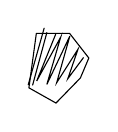
\begin{tikzpicture}[scale=.43,line cap=round]
\draw (.12,2.1)--(1.10,2.10)--(1.67,1.37)--(1.42,.78)--(.70,.04)--(-.10,.49)--(.12,2.1);
\draw (.35,2.25)--(-.12,.58) (.43,2.12)--(.01,.57) (.69,2.07)--(.13,.69)--(.84,1.99)--(.43,.59)--(1.11,2.02)--(.72,.64)--(1.35,1.63)--(1.05,.76)--(1.51,1.38);
\end{tikzpicture}}

donné par

\[
\left\{\begin{aligned}
\tau_{\infty}&\longmapsto\inserted{r_\infty=}\begin{pmatrix}-1&0\\0&1\end{pmatrix}=\tau_\infty\\
\tau_0&\longmapsto\inserted{r_0=}\begin{pmatrix}0&1\\1&0\end{pmatrix}=\tau'_\infty\\
\tau_1&\longmapsto\inserted{r_1=}\begin{pmatrix}-1&\deleted{\unsure{-}}1\\0&1\end{pmatrix}=-\tau'_0
\end{aligned}\right.\tag*{(72)}
\]

\figure{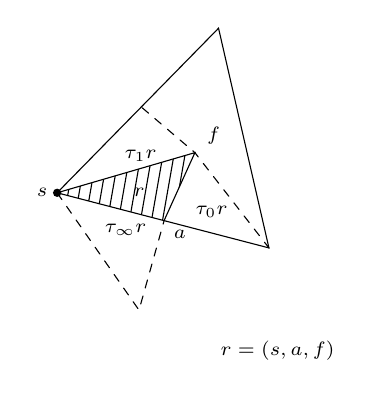
\begin{tikzpicture}[scale=1.0,line cap=round,font=\scriptsize]
\coordinate (s) at (0,.70);\coordinate (v) at (2.05,2.79);\coordinate (w) at (2.69,0);\coordinate (f) at (1.75,1.21);\coordinate (a) at (1.36,.35);\coordinate (q) at (1.04,-.79);
\draw (s)--(v)--(w)--cycle;\draw (s)--(f)--(a);
\begin{scope}\clip (s)--(f)--(a)--cycle;\foreach \x in {0,.14,...,1.75}{\draw (\x,-.1)--++(.28,1.6);}\end{scope}
\draw[dashed] (1.08,1.78)--(f)--(w) (s)--(q)--(a);
\fill (s) circle (1.5pt);\node[left] at (s) {$s$};\node[right] at (1.78,1.43) {$f$};\node[below right] at (a) {$a$};
\node at (1.04,.71) {$r$};\node at (1.06,1.17) {$\tau_1r$};\node at (1.96,.46) {$\tau_0r$};\node at (.87,.23) {$\tau_\infty r$};
\node at (2.80,-1.31) {$r=(s,a,f)$};
\end{tikzpicture}}

\margin{Cf ``formulaire pour $\unsure{\pi_{03}|\mathrm{T}_{03}|\mathrm{Th}_{03}}$ etc''}

% archive sheet number: 27
\scanpage{29}

\inserted{Ceci rappelé,} Soit \deleted{\unsure{m}}Maintenant $M$ un $\Lambda$-module libre de rang $2$, et considérons l'ens.

\[
\operatorname{Rep}(M)'\simeq\operatorname{Isom}_\Lambda(\Lambda^2,M)/\underset{\deleted{\unsure{3}}}{\pm}1\tag*{(73)}
\]

qui est un torseur \inserted{à droite} sous $\mathrm{GL}(2,\Lambda)/{\pm1}$. Comme l'hom canonique

\[
\mathbb{Z}\unsure{\mathbin{-}|\longrightarrow}\Lambda
\]

définit des hom correspondants

\[
\left\{\begin{aligned}
\mathrm{GL}(2,\mathbb{Z})&\longrightarrow\deleted{\unsure{\mathrm S}}\mathrm{GL}(2,\Lambda)\\
\mathrm{GL}(\unsure{n|2},\mathbb{Z})'&\longrightarrow\deleted{\unsure{\mathrm S}}\mathrm{GL}(n,\Lambda)'=\mathrm{GL}(2,\Lambda)/\{\pm1\}
\end{aligned}\right.\tag*{(74)}
\]

on peut considérer $\operatorname{Rep}(M)'$ comme un ensemble sur lequel $\mathrm{GL}(2,\mathbb{Z})'$ opère à droite, donc à gauche si on y tient par la modification habituelle $g\longmapsto g^{-1}$.

Donc $\operatorname{Rep}(M)'$ définit une structure \inserted{$2$-polyèdrale} triangulée (pas néc. finie) qu'il faudrait expliciter en termes des constructions du \S\ I. On peut aussi, \deleted{\unsure{gardant|prenant}} \inserted{regarder} la restriction de l'opération précédente à $\mathrm{SL}(2,\mathbb{Z})'$, on trouve une structure $2$-polyèdrale triangulée orientée (qui, pour

% archive sheet number: 28
\scanpage{30}

\mspage{14}

les \unsure{solides|soides|valeurs} généraux, s'identifie au revêtement des orientations locales du précédent). Quand on se donne une jauge $e_M\in(\det M)^*$, on peut aussi considérer l'ens des repères symplectiques

\[
\underset{\substack{\shortparallel\\\mathrm{Rep.sp.}_\Lambda(M,e_M)/\{\pm\mathrm{id}_M\}}}{\operatorname{Repsp}_\Lambda(M,e_M)'}\subset\operatorname{Rep}_\Lambda(M)'\tag*{(75)}
\]

qui est un torseur sous $\mathrm{SL}(2,\Lambda)'$, et qui devient donc un ens. sur lequel $\mathrm{SL}(2,\mathbb{Z})'$ opère. Il lui correspond donc une structure $2$-polyédrale orientée, qu'il faudrait encore expliciter en termes des constructions \unsure{précédantes|précédentes} \deleted{\unsure{d}}(du \S\ I). Sauf erreur, pour $\Lambda$ de la forme $\mathbb{Z}$ ou $\mathbb{Z}/n\mathbb{Z}$ (ce qui est nécessaire pour que lesdites constructions fournissent bien un polyèdre, au sens strict \unsure{du terme|des termes}), on retrouve,

% archive sheet number: 29
\scanpage{31}

à isom. canonique près, \inserted{qu'il faudrait expliciter} le $2$-polyèdre triangulé orienté $SP_M$. Dans ce cas d'ailleurs, l'hom qui correspond à (\unsure{75|74})

\[
\mathrm{SL}(2,\mathbb{Z})'\unsure{\mathbin{-}|\longrightarrow}\mathrm{SL}(2,\Lambda)'\tag*{(76)}
\]

% slanted
\margin{\uline{à vérifier !}}

est un hom surjectif, de sorte qu'il est clair a priori que la structure $2$-polyèdrale associée doit être connexe, et bien sûr régulière (dans le cas général, si $\Lambda_0$ est l'image de $\mathbb{Z}$ dans $\Lambda$, les composantes connexes de la structure obtenue doivent être des polyèdres triangulés réguliers, \deleted{dont la} \inserted{isomorphes} \deleted{\unsure{ayant un support et}} \inserted{entre eux, ayant} comme groupe d'automorphismes \inserted{directs} le groupe $\mathrm{SL}(2,\Lambda_0)'$.

% archive sheet number: 30
\scanpage{32}

\mspage{15}

Considérons un module libre \inserted{$M$,} \deleted{\unsure{de r|de}} \deleted{\unsure{\illegible{1}|de}} rang $2$ sur l'anneau $\Lambda=\Lambda_0$ $(\simeq\mathbb{Z}$ ou $\mathbb{Z}/n\mathbb{Z}$, $n\geq3)$, \deleted{et considérons} muni d'une jauge $e_M\in(\det M)^*$, d'où un \unsure{$2$|$1$}-polyèdre régulier triangulé $SP_M$.

Choisissons un repère \deleted{direct} de $SP_M$, \deleted{qui} \deleted{est donc} \inserted{ou} ce qui revient au même, \unsure{une|un} triplet d'éléments distincts de $S_M=M^*/{\pm1}$

\[
(s,t,u)\quad\text{tel que }\deleted{\unsure{\}}}\{s,t,u\}\in SF_M\tag*{(77)}
\]

i.e. tel qu'il existe

\[
\left\{\begin{aligned}
&(x,y,z)\in B_{\deleted{\unsure{\mathrm{sp}}}}(M)\qquad
\left[\begin{aligned}
&\text{donc}\quad\deleted{x+y}\ \inserted{(x,y)\in\operatorname{Rep}(M)}\\
&\qquad x+y+z=0\quad\text{i.e.}\quad z=-(x+y)\\
&\qquad\qquad\deleted{\text{\unsure{d'où}}}
\end{aligned}\right.\\
&\text{avec}\\
&s=\dot{x},\ t=\dot{y},\ u=\dot{z}=(x+y)^{\unsure{\bullet|\cdot}},\quad x\wedge y\in\{\pm e_M\}
\end{aligned}\right.\tag*{(78)}
\]

le repère correspondant étant

\[
r=(s,a,f),\quad\text{avec}\quad a=\{s,t\},\quad f=\{s,t,u\}\;.\tag*{(79)}
\]

\deleted{Le triplet} Supposons que le repère soit direct, i.e la base $(x,y)$ soit directe

\[
x\wedge y=e_M\;.\tag*{(80)}
\]

On va expliciter les automorphismes $\tau_0^r,\tau_1^r,\tau_\infty^r$ du polyèdre régulier $SF_M$, qui correspondent au repère \inserted{(direct)} choisi $r$ (79), i.e. à la base symplectique $(x,y)$ de $M$. (Le choix \deleted{direct} du repère direct revient à celui du choix de la base symplectique, \uline{modulo} signe.)

% archive sheet number: 31
